\documentclass{beamer}

\mode<presentation> {

% The Beamer class comes with a number of default slide themes
% which change the colors and layouts of slides. Below this is a list
% of all the themes, uncomment each in turn to see what they look like.

%\usetheme{default}
%\usetheme{AnnArbor}
%\usetheme{Antibes}
%\usetheme{Bergen}
%\usetheme{Berkeley}
%\usetheme{Berlin}
%\usetheme{Boadilla}
%\usetheme{CambridgeUS}
%\usetheme{Copenhagen}
%\usetheme{Darmstadt}
%\usetheme{Dresden}
%\usetheme{Frankfurt}
%\usetheme{Goettingen}
%\usetheme{Hannover}
%\usetheme{Ilmenau}
%\usetheme{JuanLesPins}
%\usetheme{Luebeck}
\usetheme{Madrid}
%\usetheme{Malmoe}
%\usetheme{Marburg}
%\usetheme{Montpellier}
%\usetheme{PaloAlto}
%\usetheme{Pittsburgh}
%\usetheme{Rochester}
%\usetheme{Singapore}
%\usetheme{Szeged}
%\usetheme{Warsaw}

% As well as themes, the Beamer class has a number of color themes
% for any slide theme. Uncomment each of these in turn to see how it
% changes the colors of your current slide theme.

%\usecolortheme{albatross}
%\usecolortheme{beaver}
%\usecolortheme{beetle}
%\usecolortheme{crane}
%\usecolortheme{dolphin}
%\usecolortheme{dove}
%\usecolortheme{fly}
%\usecolortheme{lily}
%\usecolortheme{orchid}
%\usecolortheme{rose}
%\usecolortheme{seagull}
%\usecolortheme{seahorse}
%\usecolortheme{whale}
%\usecolortheme{wolverine}

%\setbeamertemplate{footline} % To remove the footer line in all slides uncomment this line
%\setbeamertemplate{footline}[page number] % To replace the footer line in all slides with a simple slide count uncomment this line

%\setbeamertemplate{navigation symbols}{} % To remove the navigation symbols from the bottom of all slides uncomment this line
}

\usepackage{graphicx} % Allows including images
\usepackage{booktabs} % Allows the use of \toprule, \midrule and \bottomrule in tables
\usepackage[utf8]{inputenc}
\usepackage{float}
\usepackage{subcaption}

%----------------------------------------------------------------------------------------
%	TITLE PAGE
%----------------------------------------------------------------------------------------

\title[A Fast Approximation of WL RDF kernel]{A Fast Approximation of the Weisfeiler-Lehman Graph Kernel for RDF Data}
\subtitle{Advanced Algorithms and Graph Minings}
\author{Lorenzo Palloni \and Emilio Cecchini}
\institute[]{
    Università Degli Studi di Firenze \\
    \medskip
    \textit{lorenzo.palloni@stud.unifi.it \and emilio.cecchini@stud.unifi.it}
}
\date{\today}

\begin{document}

\begin{frame}
\titlepage % Print the title page as the first slide
\end{frame}

%----------------------------------------------------------------------------------------
%	PRESENTATION SLIDES
%----------------------------------------------------------------------------------------

\begin{frame}
\frametitle{Introduction}

\begin{itemize}
\item
In order to apply machine learning algorithms on graphs it is necessary to develop algorithms to compute how similar two graphs are.

\item
Starting from the well-known Weisfeiler-Lehman isomorphism test, they have been developed kernel methods to measure the similarity between graphs.

\item
This paper proposes a fast approximation of a Weisfeiler-Lehman kernel applied to RDF data.


\end{itemize}

\end{frame}

\begin{frame}
\frametitle{Graph Kernels}

Kernel-based machine learning algorithms abandon the explicit vector representations of data items by means of the \textit{kernel function}.

\begin{definition}[Graph Kernel]
Let $\mathbb{G}$ be a non-empty set of graphs. Any function $k: \mathbb{G} \times \mathbb{G} \rightarrow \mathbb{R}$ that takes as input two graphs $G$ and $G^\prime$ and returns a real number that is equal to the scalar product between $G$ and $G^\prime$ in a (even unknown) feature space is a valid kernel function.
\end{definition}

\end{frame}

%------------------------------------------------

\begin{frame}
\frametitle{Graphs isomorphism}

\begin{itemize}
\item
Two graphs $G$ and $G^\prime$ are isomorphic if exists a bijective mapping between the labels of $G$ to the label of $G^\prime$

\item
The graph isomorphism problem is NP.

\item
The graph kernel introduced in this paper uses concepts from the \textit{Weisfeiler-Lehman test} of isomorphism.
\end{itemize}

\end{frame}

%------------------------------------------------

\begin{frame}
\frametitle{Weisfeiler-Lehman test}

\begin{itemize}
\item
Assume we are given two graphs $G$ and $G^\prime$ and we would like to test whether they are isomorphic.
\item
The Weisfeiler-Lehman test performs $h$ iterations.
\item
The key idea of the algorithm is to augment the node labels by the sorted set of node labels of neighbouring nodes, and compress these augmented labels into new, short labels.
\item
These steps are then repeated until the node label sets of $G$ and $G^\prime$ differ, or the number of iterations reaches $h$.
\item
The runtime complexity of the Weisfeiler-Lehman algorithm with h iterations is $O(hk)$, where $k$ is the number of labels in $G$ and $G^\prime$.
\end{itemize}

\end{frame}

%------------------------------------------------

\begin{frame}
\frametitle{Weisfeiler-Lehman test}

\begin{center}
\begin{figure}
\end{figure}
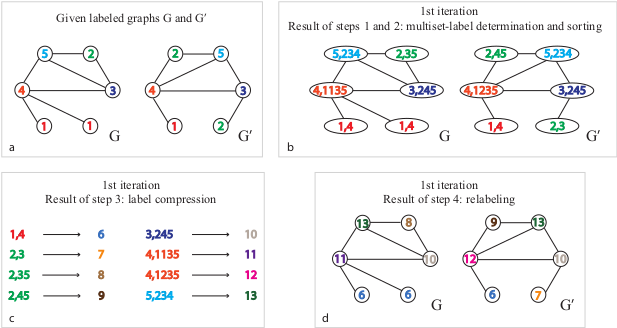
\includegraphics[width=\textwidth]{img/wl_iteration_upper.png}
\end{center}

\end{frame}

%------------------------------------------------

\begingroup
\small
\begin{frame}
\frametitle{Weisfeiler-Lehman kernel}

\begin{definition}[Weisfeiler-Lehman kernel]
Let $G_i = (V, E, l_i)$ and $G_i^\prime = (V^\prime , E^\prime , l_i)$ be the i-th iteration rewriting of the graphs $G$ and $G^\prime$ with the Weisfeiler-Lehman algorithm and h the number of iterations. Then the Weisfeiler-Lehman kernel is defined as:

\begin{align}
k_{\mathrm{WL}}^{h}\left(G, G^\prime\right)=\sum_{i=0}^h k_\delta\left(G_i, G_i^\prime\right)
\end{align}

where

\begin{align}
k_\delta\left((V, E, l),\left(V^\prime, E^\prime, l^\prime\right)\right)=\sum_{v \in V} \sum_{v^{\prime} \in V^{\prime}} \delta\left(l(v), l^{\prime}\left(v^{\prime}\right)\right)
\end{align}

Here $\delta$ is the Dirac kernel, which tests for equality, it is 1 if its arguments are equal, and 0 otherwise.
\end{definition}

\end{frame}
\endgroup

%------------------------------------------------

\begin{frame}
\frametitle{Weisfeiler-Lehman Subtree Kernel}

\begin{center}
\begin{figure}
\end{figure}
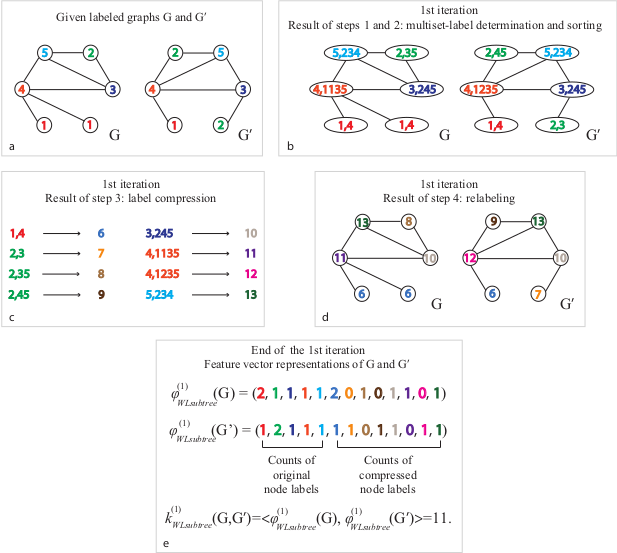
\includegraphics[width=\textwidth,height=0.8\textheight,keepaspectratio]{img/wl_iteration_total.png}
\end{center}

\end{frame}

%------------------------------------------------

\begin{frame}
\frametitle{The Resource Description Framework}

\begin{itemize}
\item
The Resource Description Framework (RDF) is the foundation for knowledge representation on the semantic web.

\item
It is based on the  idea of making statements about resources in a \textit{subject-predicate-object} form, called \textit{triples}

\item
A set of triples represents a graph, that has subjects and objects as nodes and predicates as edges (note that is a \textit{directed multigraph with labeled edges}).
\end{itemize}

\end{frame}

%------------------------------------------------

\begin{frame}
\frametitle{The Resource Description Framework}

\begin{center}
\begin{figure}
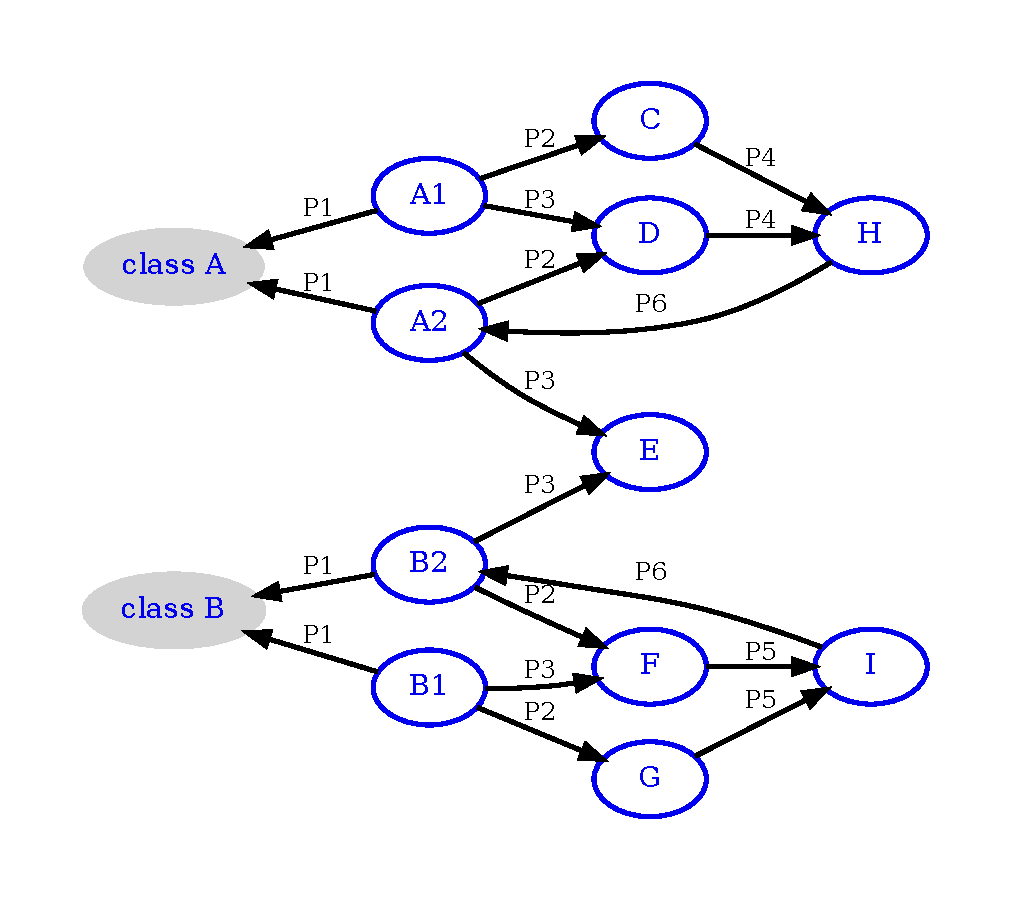
\includegraphics[scale=0.55,keepaspectratio]{img/07-Graph}
\end{figure}
\end{center}

\end{frame}

%------------------------------------------------

\begin{frame}
\frametitle{Fast Weisfeiler-Lehman for RDF}

\begin{itemize}
\item
The most immediate approach to apply graph kernels to RDF is to extract subgraphs for the instances that we are interested in and to compute the kernel on these subgraphs.

\item
Potentially it can be more efficient to do the kernel computation directly on the larger underlying RDF graph, instead of extracting many subgraphs.

\item
This paper proposes an approximation of the Weisfeiler-Lehman kernel designed for RDF data.
\end{itemize}

\end{frame}

%------------------------------------------------

\begin{frame}
\frametitle{Weisfeiler-Lehman RDF graph}

\begin{definition}[Weisfeiler-Lehman RDF graph]
A Weisfeiler-Lehman RDF graph is a graph $G = (V, E, l)$, where $V$ is a set of vertices, $E$ a set of directed edges, and $l:(V \cup E) \times N \rightarrow \Sigma$ a labeling function from vertices $V$ or edges $E$ and a depth index $j \in \mathbb{N}$ to a set of labels $\Sigma$.
\end{definition}

\begin{definition}[Neighborhood]
The neighborhood $N(v) = \{(v^\prime, v) \in E\}$ of a vertex is the set of edges going to the vertex $v$ and the neighborhood $N((v, v^\prime)) = {v}$ of an edge is the vertex that the edge comes from.
\end{definition}

\end{frame}



\begin{frame}
\frametitle{Graph extraction from RDF}

\begin{itemize}
\item
Given a set of RDF triples and a set of instances I, there is an algorithm to build a Weisfeiler-Lehman RDF graph.

\item
For each instance $i$ a subgraph up to depth $d$ is extracted from the RDF dataset and this subgraph is added to the total graph G that the algorithm is building. Thus, vertices and edges are only added if they have not been added to the graph already.

\item
Next to the graph G we also construct mappings $\mathcal{V}_i$ and $\mathcal{E}_i$ for each instance $i$, which records which vertices and edges belong to the subgraph of instance $i$ at which depth.
\end{itemize}

\end{frame}


\begingroup
\small
\begin{frame}
\frametitle{Graph extraction from RDF}

Extraction of the instances A1 and B1.

\begin{center}
\begin{figure}
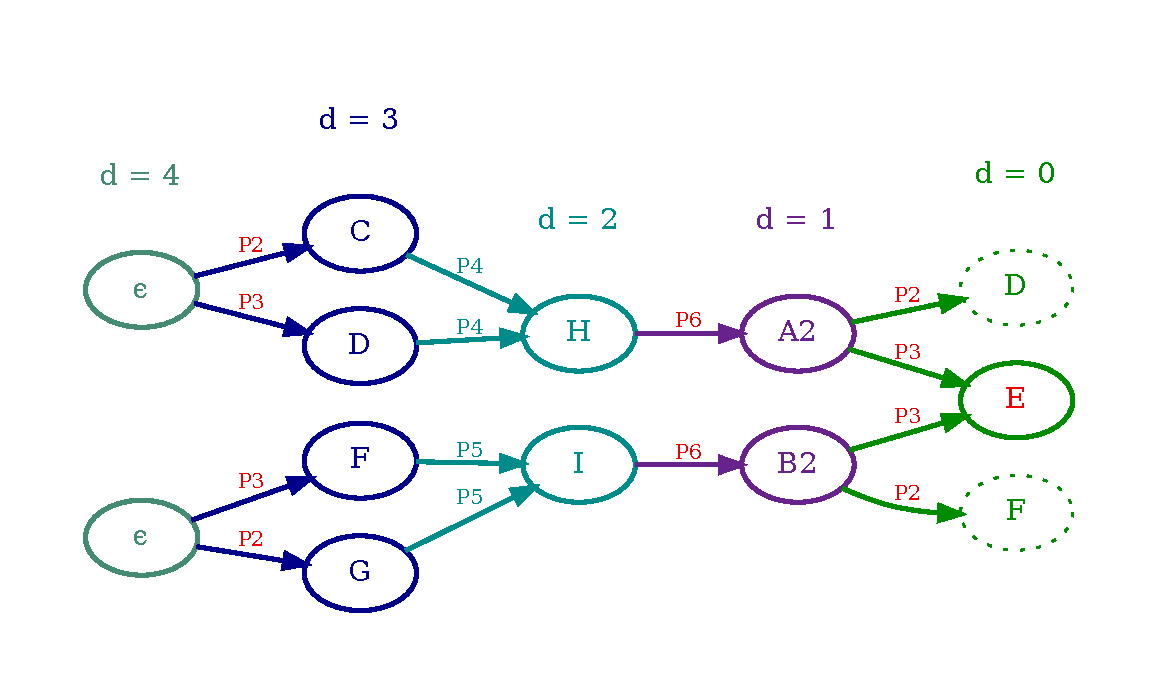
\includegraphics[width=\textwidth,keepaspectratio]{img/07-subGraph_A1_B1}
\end{figure}
\end{center}

\end{frame}
\endgroup


\begin{frame}
\frametitle{Relabeling of the Weisfeiler-Lehman RDF graph}

\begin{itemize}
\item
The relabeling process is quite similar to the standard one.

\item
It is extended to directed and labeled edges.

\item
The augmented labels are constructed taking into account the new definition of neighborhood and the depths.
\end{itemize}

\end{frame}

%----------------------------------------------------------------------------

\begingroup
\small
\begin{frame}
\frametitle{Relabeling of the Weisfeiler-Lehman RDF graph}

Label propagation.

\begin{center}
\begin{figure}
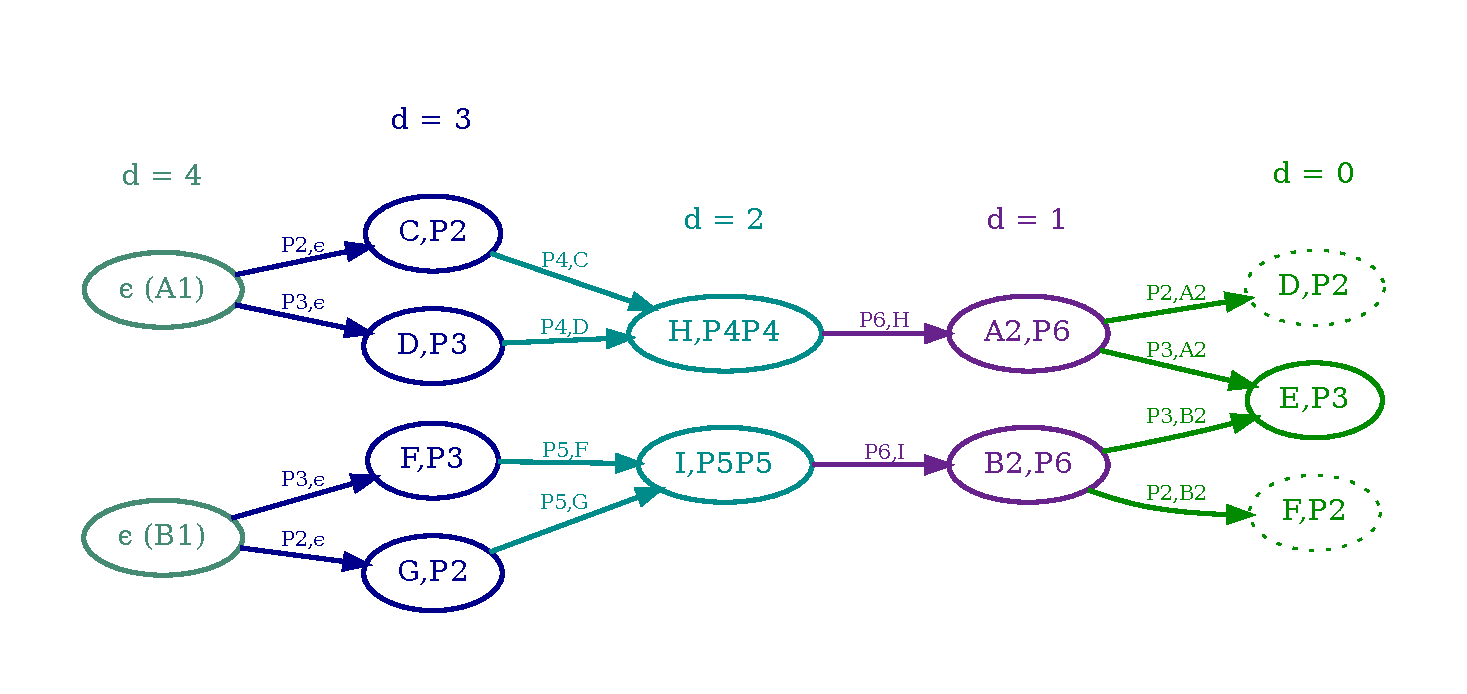
\includegraphics[width=\textwidth,keepaspectratio]{img/07-almost_relabeled}
\end{figure}
\end{center}

\end{frame}
\endgroup

%----------------------------------------------------------------------------

\begingroup
\small
\begin{frame}
\frametitle{Relabeling of the Weisfeiler-Lehman RDF graph}

Relabeling.

\begin{center}
\begin{figure}
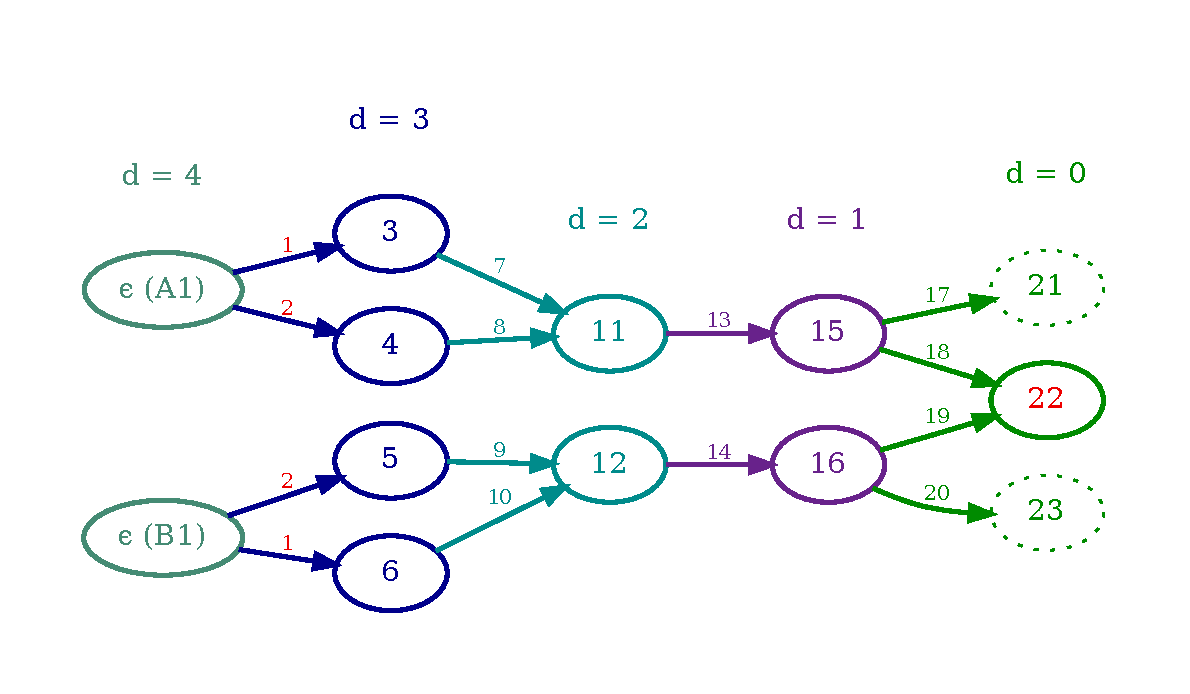
\includegraphics[width=\textwidth,keepaspectratio]{img/07-relabeled}
\end{figure}
\end{center}

\end{frame}
\endgroup

%----------------------------------------------------------------------------

\begingroup
\small
\begin{frame}
\frametitle{Weisfeiler-Lehman kernel for RDF}

\begin{definition}[Weisfeiler-Lehman kernel for RDF]
Let $G$ be a Weisfeiler-Lehman RDF graph and rewritten for h iterations, and $l_0$ to $l_h$ the resulting label functions. Then we compute a kernel between two instances $i$, $i^\prime \in I$, as:

\begin{align}
k_{\mathrm{WLRDF}}^{h}\left(i, i^{\prime}\right)=\sum_{n=0}^{h} \frac{n+1}{h+1} k_{\delta, \mathrm{RDF}}^{n}\left(\left(\mathcal{V}_{i}, \mathcal{E}_{i}\right),\left(\mathcal{V}_{i^{\prime}}, \mathcal{E}_{i^{\prime}}\right)\right)
\end{align}

where

\begin{align}
k_{\delta, \mathrm{RDF}}^{n}\left(\left(\mathcal{V}_{i}, \mathcal{E}_{i}\right),\left(\mathcal{V}_{i^{\prime}}, \mathcal{E}_{i^{\prime}}\right)\right) &=\sum_{(v, d) \in \mathcal{V}_{i}\left(v^{\prime}, d^{\prime}\right) \in \mathcal{V}_{i^{\prime}}} \delta\left(l_{n}(v, d), l_{n}\left(v^{\prime}, d^{\prime}\right)\right) \\
&+\sum_{(e, d) \in \mathcal{E}_{i}\left(c^{\prime}, d^{\prime}\right) \in \mathcal{V}_{i^{\prime}}} \delta\left(l_{n}(e, d), l_{n}\left(e^{\prime}, d^{\prime}\right)\right)
\end{align}

\end{definition}

\end{frame}
\endgroup

%------------------------------------------------

\begingroup
\footnotesize
\begin{frame}
\frametitle{Weisfeiler-Lehman kernel for RDF}

\begin{exampleblock}{Example}
\begin{align*}
k_{\mathrm{WLRDF}}^h\left(A1, B1\right) &= \sum_{n=0}^h \frac{n+1}{h+1} k_{\delta, \mathrm{RDF}}^{n}\left(\left(\mathcal{V}_{A1}, \mathcal{E}_{A1}\right),\left(\mathcal{V}_{B1}, \mathcal{E}_{B1}\right)\right) = \dfrac{1}{2} \cdot 10 + \dfrac{2}{2} \cdot 3 = 8
\end{align*}
\end{exampleblock}

\begin{figure}
\centering
\begin{subfigure}{.5\textwidth}
    \centering
    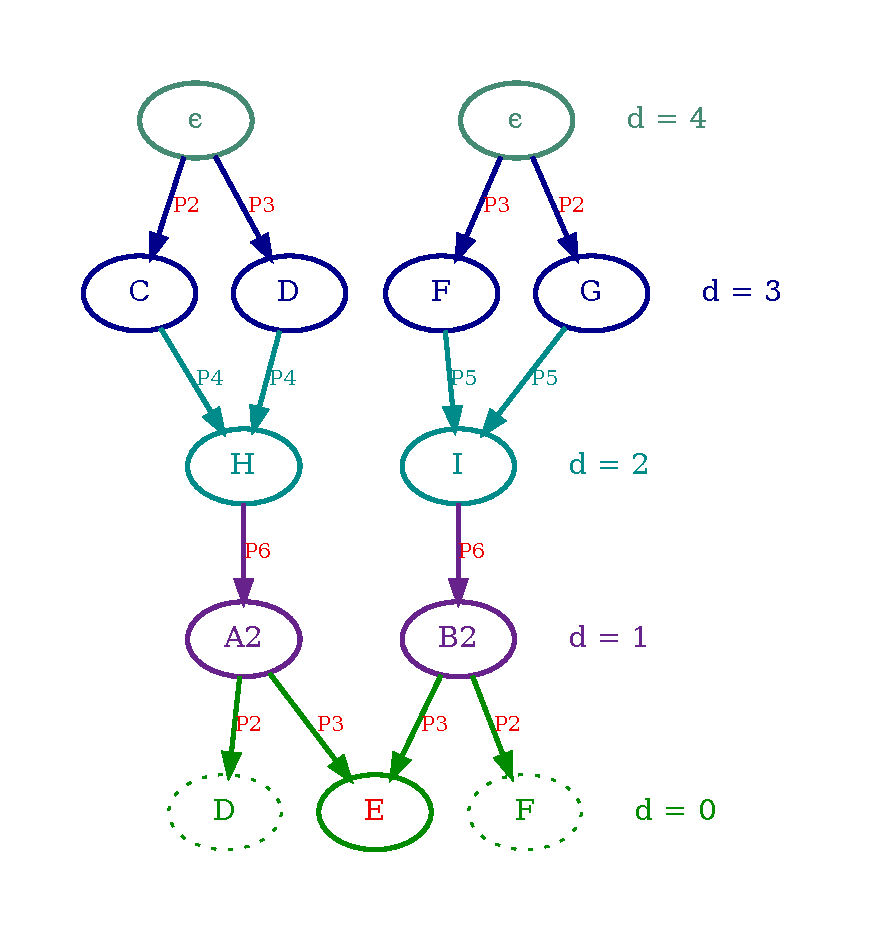
\includegraphics[width=0.9\linewidth]{img/07-subGraph_A1_B1_vertical}
\end{subfigure}%
\begin{subfigure}{.5\textwidth}
    \centering
    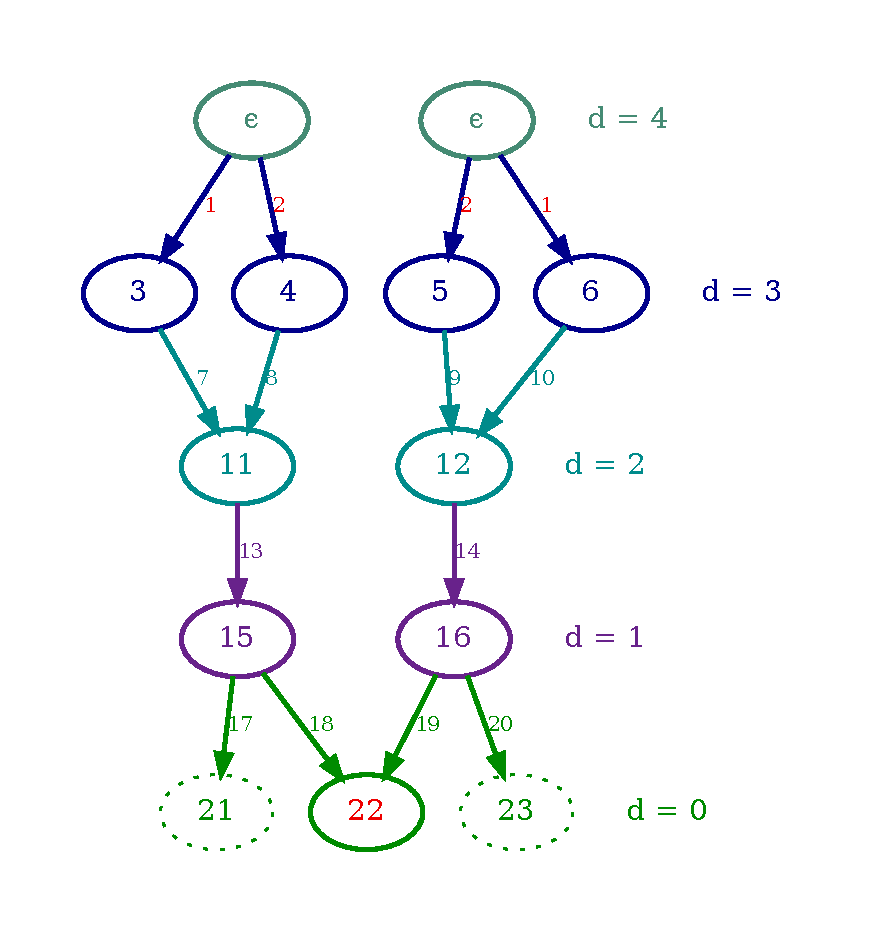
\includegraphics[width=0.9\linewidth]{img/07-relabeled_vertical}
\end{subfigure}
\end{figure}

\end{frame}
\endgroup
%------------------------------------------------

\begin{frame}
\frametitle{Complexity}

\begin{itemize}
\item
The complexity of the standard relabeling algorithm on a set of graphs is O$(Nh(n + m))$, where $N$ is the number of graphs, $h$ is the number of iterations and $n$ and $m$ are the number of vertices and edges per graph.
\item
This new relabeling method does not have $N$ graphs, but it introduces $d$ labels per vertex/edge, where $d$ is the extraction depth.
\item
If the WL RDF graph has $k$ nodes and edges the complexity of this new algorithm is $O(dhk)$
\item
The new proposed method is faster than the regular one if $hk < N(n+m)$
\end{itemize}

\end{frame}

%------------------------------------------------

\begingroup
\footnotesize
\begin{frame}
\frametitle{References}

\begin{thebibliography}{99} % Beamer does not support BibTeX so references must be inserted manually as below

\bibitem{lamport94}
    Vries Gerben Klaas Dirk,
    A Fast Approximation of the Weisfeiler-Lehman Graph Kernel for RDF Data,
    2013

\bibitem{wl-kernels}
    Shervashidze, N., Schweitzer, P., van Leeuwen, E.J., Mehlhorn, K., Borgwardt, K.M.
    Weisfeiler-lehman graph kernels,
    2011
\end{thebibliography}

\end{frame}
\endgroup

%------------------------------------------------

\end{document}
